\startchapter{Simplified Molecular Model}
\label{chapter:simplified_molecular_model}

\section{Description}
In the last chapter, we have seen how IR, Raman and SFG spectres are produced theoretically. However, before we jump to the real molecule models, we would like to study the properties of our LP model first. We have encountered cases when LP model failed to give us the expected composition, and this is actually the most case. We want to know why and when our LP model would fail?

Therefore, we constructed a toy molecule model to study our LP model first, meanwhile, get a better understanding of the spectroscopy techniques.

For this toy model, we use the following equation to generate the IR spectroscopy, 
\begin{eqnarray}
& f_{\theta}(x) = \displaystyle\sum^{4}_{q=1} A_q^2 * cos^2(\theta - \theta_q)\frac{\gamma^2}{(x- w_q)^2 + \gamma^2} \nonumber \\
& A:~amplitude \nonumber \\
& \theta_q : angle \nonumber \\
& \gamma: width \nonumber \\
& w_q : frequency \nonumber 
\end{eqnarray}

This is the cosine projection of the IR spectra. Furthermore, this molecule only contains 4 vibration modes, with the peaks happen at frequency of 2850, 2960, 3050 and 3200, and the widths for the peaks are 5, 10, 5 and 15, and the heights, which are 1, 0.7, -0.2 and 0.5 respectively. The comparing angle for each peak( What does those angle refer???) is 15, 90, 0 and 60. We generate 10 candidate spectra with 10 different $\theta$ values:
$\theta = 0^{\circ}, 10^{\circ}, 20^{\circ}, 30^{\circ}, 40^{\circ}, 50^{\circ}, 60^{\circ}, 70^{\circ}, 80^{\circ}, 90^{\circ} $ \\

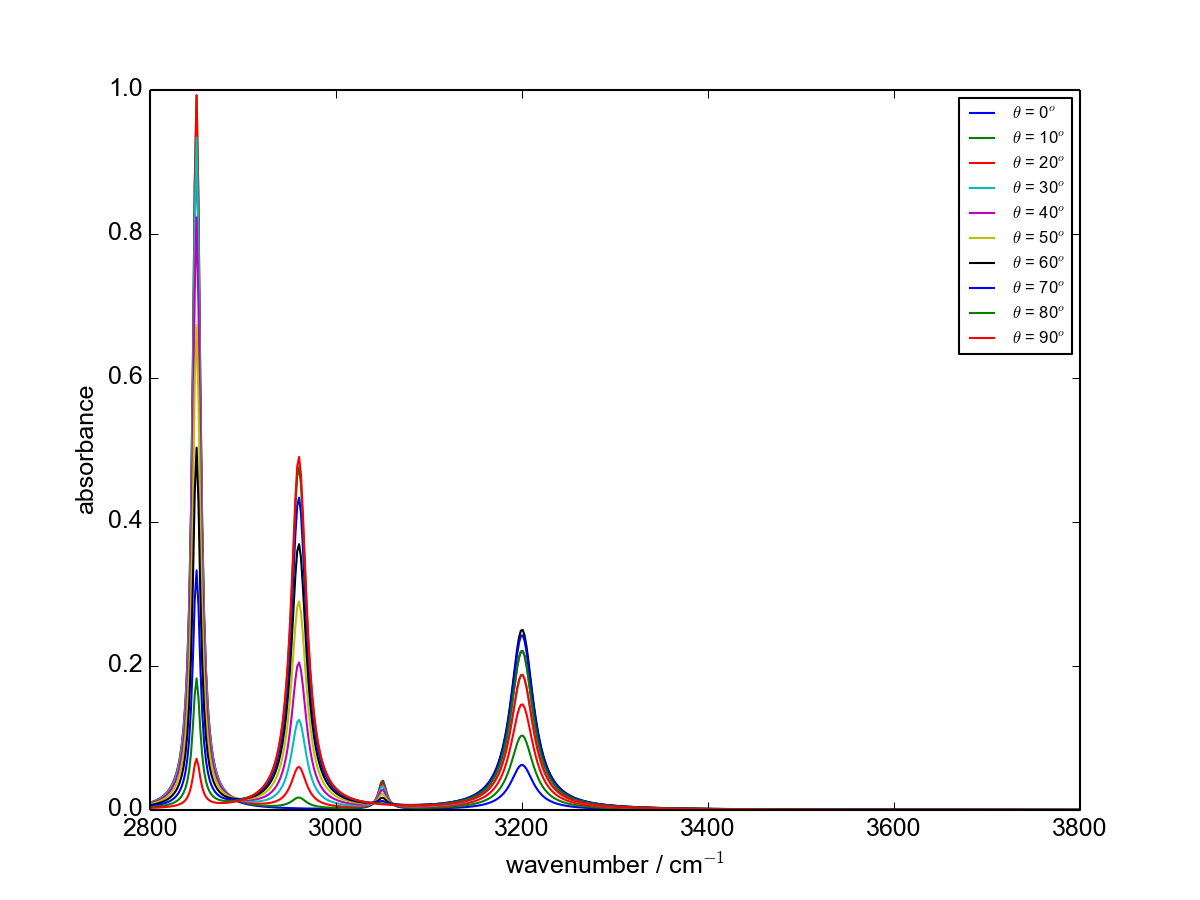
\includegraphics[scale=0.7]{Toy_Model_IR_Cosine_Projection.png}

As you can see from the graph that, these 10 candidates have peaks at the same frequency. And the only difference on $\theta$ makes them very similar to each other. This also makes it really difficult to obtain exact composition for the targeted spectrum, as various combinations of candidates are possible to achieve the targeted spectrum.

As an example, we compose a target spectrum by combining 15 percent $\theta$ of 20 degree's spectrum and 85 percent of $\theta$ of 70 degree's spectrum: $0.15*f_{20}(x) + 0.85*f_{70}(x)$. \\

\section{Linear Programming Model for Spectra Study}

The linear programming model that we construct to check if the optimal solution returned actually match the known composition is as following. The model has used in the studies of \cite{03}  and \cite{04}. \\
\begin{eqnarray}
& minimize \displaystyle\sum^{points}_{p=1} \left| Target- \displaystyle\sum^{candidates}_{c=1}p_{c}f_{\theta}(x) \right| \nonumber \\
& p_c: percentage ~of~ each~ candidate \nonumber \\
& p: number~ of~ points~ selected~ both~ from~ candidates~ and~ Target \nonumber 
\end{eqnarray}
 
In this model, the unknown percentage of each candidate is the decision variable, it is denoted by $p_c$. We select data points along the wavelength frequency,the data point is denoted by $p$ here. Based on each data point, we calculate the absolute residual between target spectrum and the one composed by the decision variables. Then the objective function is to minimize of the sum of the absolute residual over all the data points. \\

However, in order to actually apply Linear Programming, we need to get rid of the absolute sign in the objective function. We achieve this goal by introducing one more variable X and two more constraints for each data point. Therefore:\\

For each point:
\begin{eqnarray} 
& X = \left| Target-\displaystyle\sum^{candidates}_{c=1}p_{c}f_{\theta}(x) \right| \nonumber \\
&  X \geq Target-\displaystyle\sum^{candidates}_{c=1}p_{c}f_{\theta}(x)   \nonumber \\
& X \geq -Target+\displaystyle\sum^{candidates}_{c=1}p_{c}f_{\theta}(x)  \nonumber
\end{eqnarray} 

We then convert the previous model into one that can actually be solved by Linear Programming solver:\\

\begin{eqnarray} 
& minimize \displaystyle\sum^{points}_{p=1} X_p \nonumber \\
& X_1 - Target_1 + \displaystyle\sum^{candidates}_{c=1}p_{c}f_{\theta}(x_1) \geq 0 \nonumber \\
& X_1 + Target_1 - \displaystyle\sum^{candidates}_{c=1}p_{c}f_{\theta}(x_1) \geq 0 \nonumber \\
& ... \nonumber \\
& X_n - Target_n + \displaystyle\sum^{candidates}_{c=1}p_{c}f_{\theta}(x_n) \geq 0 \nonumber \\
& X_n + Target_n - \displaystyle\sum^{candidates}_{c=1}p_{c}f_{\theta}(x_n) \geq 0 \nonumber \\
& \displaystyle\sum^{candidates}_{c=1}p_{c} = 1 \nonumber
\end{eqnarray} 

The last equality restrict the sum of the percentage to 1.



  

\section{Experiments}

\subsection{Experiment 1 and 2 Setting}
\begin{table}
\begin{tabular}{l | l | l | l }
\hline
Experiment index & 1 & 2  \\
\hline
Number of Candidates & 4 & 4  \\
\hline
Candidates & [0, 10, 20, 30] & [0, 5, 10, 15] \\
\hline
Target Composition & [0.1, 0.5, 0.4, 0] & [0.1, 0.5, 0.4, 0]     \\
\hline
Number of Constraints & 100(cos) &  100(cos)     \\
\hline
Return Composition & [0.1, 0.5, 0.4, 0] & [0, 0.796962, 0.103038, 0.1] \\
\hline
\end{tabular} 
\end{table}	

\subsection{Experiment 2 Result Plotting}
%\includegraphics[scale=0.3]{result_plotting_ir_cos_4candi_1.png}\\
The spectroscopy of result composition is almost identical with the target one. Therefore, the LP solver has achieved its optimal.


\subsection{Experiment 3 Setting}

\begin{table}
\begin{tabular}{l | p{7cm} | }
\hline
Experiment index & 3  \\
\hline
Number of Candidates & 10   \\
\hline
Candidates & [0, 10, 20, 30, 40, 50, 60, 70, 80, 90]  \\
\hline
Target Composition & [0.1, 0, 0.5, 0, 0.4, 0, 0, 0, 0, 0] \\
\hline
Number of Constraints & 100(cos) \\
\hline
Return Composition & [0, 0, 0.730541, 0, 0.212061,0, 0, 0.0573978, 0, 0] \\
\hline
\end{tabular} 
\end{table}	


\subsection{Experiment 3 Result Plotting}


%\includegraphics[scale=0.3]{result_plotting_ir_cos_10candi_1.png} \\
The spectroscopy of result composition is almost identical with the target one. Therefore, the LP solver has achieved its optimal.


\subsection{Experiment 4 Setting}

\begin{table}
\begin{tabular}{l | p{7cm} | }
\hline
Experiment index & 4  \\
\hline
Number of Candidates & 4   \\
\hline
Candidates & [0, 5, 10, 15]  \\
\hline
Target Composition & [0.1, 0.5, 0.4, 0] \\
\hline
Number of Constraints & 100(cos) + 100(sin) \\
\hline
Return Composition & [0.1, 0.5, 0.4, 0] \\
\hline
\end{tabular} 
\end{table}		


\subsection{Experiment 5 Setting}
\begin{table}
\begin{tabular}{l | p{7cm} | }
\hline
Experiment index & 5  \\
\hline
Number of Candidates & 10   \\
\hline
Candidates & [0, 10, 20, 30, 40, 50, 60, 70, 80, 90]  \\
\hline
Target Composition & [0.1, 0, 0.5, 0, 0.4, 0, 0, 0, 0, 0] \\
\hline
Number of Constraints & 100(cos) + 100(sin) \\
\hline
Return Composition & [0.1, 0, 0.5, 0, 0.4, 0, 0, 0, 0, 0] \\
\hline
\end{tabular} 
\end{table}



\subsection{Constraint Study Based on Experiment 4}
\begin{table} \small
\begin{tabular}{l | p{3cm} | l}
	\hline
	Points & Points Selection & Result \\ \hline
	10 & [2800, 3300, 50] & [0, 0.796962, 0.103038, 0.1] \\ \hline
	20 & [2800, 3300, 25] & [0, 0.796962, 0.103038, 0.1] \\ \hline
	25 & [2800, 3300, 20] & [0, 0.796962, 0.103038, 0.1] \\ \hline
	32 & [2800, 3300, 15] & [0, 0.796962, 0.103038, 0.1] \\ \hline
	50 & [2800, 3300, 10] & [0, 0.796962, 0.103038, 0.1] \\ \hline
	100 & [2800, 3300, 5] & [0, 0.796962, 0.103038, 0.1] \\ \hline
	$100 + 1$ & [2800, 3300, 5], [2800, 3300, 500] & [0, 0.796962, 0.103038, 0.1] \\ \hline
	$100 + 5$ & [2800, 3300, 20], [2800, 3300, 100] & [0, 0.796962, 0.103038, 0.1] \\ \hline
	$100 + 10$ & [2800, 3300, 20], [2800, 3300, 50] & [0, 0.796962, 0.103038, 0.1] \\ \hline
	$100 + 50$ & [2800, 3300, 20], [2800, 3300, 10] & [0.1, 0.5, 0.4, 0] \\ \hline
	$100 + 100$ & [2800, 3300, 20], [2800, 3300, 5] & [0.1, 0.5, 0.4, 0] \\ 
	\hline
\end{tabular} 
\end{table}



\subsection{Constraint Study Based on Experiment 4}
Result:[0, 0.796962, 0.103038, 0.1]\\
Target: [0.1, 0.5, 0.4, 0]\\
%\includegraphics[scale=0.3]{result_plotting_ir_sin_4candi_constraint_study_experiment4.png}



\subsection{Constraint Study Based on Experiment 5}
\begin{table} \tiny
\begin{tabular}{l | p{3cm}  | p{6cm}}
\hline
Points & Point Selection & Result \\ \hline
10 & [2800, 3300, 50] & [0.156758, 0, 0, 0.825977, 0, 0, 0, 0, 0, 0.017265] \\ \hline
25 & [2800, 3300, 20] & [0, 0, 0.730541, 0, 0.212061, 0, 0, 0.0573978, 0, 0, 0] \\ \hline
50 & [2800, 3300, 10] & [0, 0, 0.730541, 0, 0.212061, 0, 0, 0.0573978, 0, 0, 0] \\ \hline
100 & [2800, 3300, 5] & [0, 0, 0.730541, 0, 0.212061, 0, 0, 0.0573978, 0, 0, 0] \\ \hline
500 & [2800, 3300, 5] & [0, 0, 0.730541, 0, 0.212061, 0, 0, 0.0573978, 0, 0, 0] \\ \hline	
$100 + 1$ & [2800, 3300, 5], [2800, 3300, 500] & [0, 0, 0.730541, 0, 0.212061, 0, 0, 0.0573978, 0, 0, 0] \\ \hline
$100 + 10$ & [2800, 3300, 5], [2800, 3300, 50] & [0.361587, 0, 0.312061, 0.326352, 0, 0, 0, 0, 0] \\ \hline
$100 + 20$ & [2800, 3300, 5], [2800, 3300, 25] & [0.174023, 0, 0, 0.791447, 0, 0, 0.0345301, 0, 0, 0] \\ \hline
$100 + 25$ & [2800, 3300, 20], [2800, 3300, 20] & [0.174023, 0, 0, 0.791447, 0, 0, 0.0345301, 0, 0, 0] \\ \hline
$100 + 50$ & [2800, 3300, 5], [2800, 3300, 10] & [0, 0, 0.753209, 0, 0.146791, 0, 0.1, 0, 0, 0] \\ \hline
$100 + 84$ & [2800, 3300, 5], [2800, 3300, 6] & [0.174023, 0, 0, 0.791447, 0, 0, 0.0345301, 0, 0, 0] \\ \hline
$100 + 100$ & [2800, 3300, 5], [2800, 3300, 5] & [0.1, 0, 0.5, 0, 0.4, 0, 0, 0, 0, 0] \\ 
\hline
\end{tabular} \\
\end{table}



\subsection{Constraint Study Based on Experiment 5}
Result:[0, 0, 0.730541, 0, 0.212061,0, 0, 0.0573978, 0, 0]\\
Target: [0.1, 0, 0.5, 0, 0.4, 0, 0, 0, 0, 0]\\
%\includegraphics[scale=0.3]{result_plotting_ir_sin_10candi_constraint_study_experiment5.png}
\\
Idea: We can obtain different solutions by have different constraints, as long as the residual is smaller than the threshold we have setted up. 





\subsection{Experiment 6 Setting}
Case with 4 candidates when result composition does not match to target one: 
\begin{table} \small
\begin{tabular}{l | p{3cm} | l}
\hline
Experiment index & 6  \\
\hline
Number of Candidates & 4   \\
\hline
Candidates & [0, 10, 20, 30]  \\
\hline
Target Composition & [0.1, 0.5, 0.3, 0.1] \\
\hline
\hline
	Points & Point Selection & Result \\ \hline
	50 & [2800, 3300, 10] & [0.2, 0.212061, 0.587939, 0] \\ \hline
	100 & [2800, 3300, 5] & [0.2, 0.212061, 0.587939, 0] \\ \hline
	$100 + 50$ & [2800, 3300, 5], [2800, 3300, 10] & [0.787939, 0.0120615, 0.2, 0]\\ \hline
	$100 + 100$ & [2800, 3300, 5], [2800, 3300, 5] & [0.787939, 0.0120615, 0.2, 0] \\ 
\hline
\end{tabular} \\
\end{table}



\subsection{Experiment 7 Setting}
Case with 10 candidates when result composition does not match to target one: 
\begin{table} \tiny
\begin{tabular}{l | l | l}
\hline
Experiment index & 7  \\
\hline
Number of Candidates & 10   \\
\hline
Candidates & [0, 10, 20, 30, 40, 50, 60, 70, 80, 90]  \\
\hline
Target Composition & [0.1, 0, 0.4, 0, 0.4, 0.1, 0, 0, 0, 0] \\
\hline
\hline
	Points & Point Selection & Result \\ \hline
	100 & [2800, 3300, 5] & [0, 0, 0.731043, 0.149797, 0, 0, 0.119159, 0, 0, 0] \\ \hline
	$100 + 100$ & [2800, 3300, 5], [2800, 3300, 5] & [0.156072, 0, 0, 0.831607, 0, 0, 0, 0, 0, 0.0123217] \\ \hline
\end{tabular} \\
\end{table}



\subsection{Experiment 8 Setting}
Case with 10 candidates when result composition does not match to target one: 
\begin{table} \tiny
\begin{tabular}{l | l | l}
\hline
Experiment index & 8  \\
\hline
Number of Candidates & 10   \\
\hline
Candidates & [0, 5, 10, 15, 20, 25, 30, 35, 40, 45]  \\
\hline
Target Composition & [0.1, 0, 0.5, 0, 0.4, 0, 0, 0, 0, 0] \\
\hline
\hline
	Points & Point Selection & Result \\ \hline
	10 & [2800, 3300, 50] & [0, 0, 0.787939, 0, 0.112061, 0, 0.1, 0, 0, 0] \\ \hline
	50 & [2800, 3300, 10] & [0, 0, 0.731043, 0.149797, 0, 0, 0.119159, 0, 0, 0] \\ \hline
	100 & [2800, 3300, 5] & [0, 0, 0.731043, 0.149797, 0, 0, 0.119159, 0, 0, 0] \\ \hline
	$100 + 1$ & [2800, 3300, 5], [2800, 3300, 500] & [0, 0, 0.731043, 0.149797, 0, 0, 0.119159, 0, 0, 0] \\ \hline
	$100 + 100$ & [2800, 3300, 5], [2800, 3300, 5] & [0.156072, 0, 0, 0.831607, 0, 0, 0, 0, 0, 0.0123217] \\ \hline
\end{tabular} \\
\end{table}


\subsection
Concern(: too easy to find the case that LP solver not returning the target composition.


\section{Result}


\section{Discussion}
During the try-out, we first select the data points at the peaks, which are four points at frequency of 2850, 2960, 3050 and 3200. We then construct the Linear Programming model based on these data points. The result returned by LP-solver matched to the known one. However, if we randomly select four data points, the returned result usually does not match to the know one. At the end, we increase the number of data points, at each 5 wavelength frequency gap, a data point will be selected. And the returned result will eventually match to the known one. \\

The more data points we select, the more information about the candidates and targeted spectrum we will have in our model. Therefore, the more complicated and complete model we will construct. As we select one data point, a new variable is introduced to our model, meanwhile, two new constraints are brought into our model as well. This means that solution space is further and better restricted. When we select data points only on the peaks, these data points already contains enough information for the solver to distinguish the candidates. However, if we randomly select four data points, they may not contain enough information in order to construct the model to obtain the desired result. 
\subsection{Conclusion}
		

		 




%\input chapters/3/sec_latexhelp
